\section{Implementing a Graphical User Interface (GUI) Framework, and the Power of Lenses}
\label{sec:gui}

Gloss provided an interim layer to abstract away the complexities of OpenGL and impure drawing code, but as it turned out further abstractions on top of this were desirable. Gloss provides no ``widgets'' (buttons, scroll bars, etc), nor does it facilitate separable concerns for event handling.

\begin{marginfigure}
	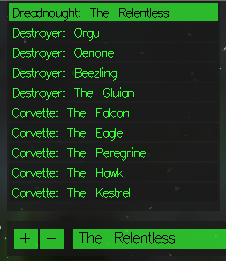
\includegraphics{res/sheen/fleetbuilder1.png}
	\caption[Fleet builder UI built using Sheen]{Part of the fleet builder UI built using Sheen.}
	\label{fig:openglbasicout}
\end{marginfigure}

Some time was spent in developing a framework on top of Gloss to enable easier construction of graphical interfaces, which has been glibly titled \emph{Sheen}\index{Sheen}. Provided by Sheen is a mechanism for event handling, recursively nested views, and various pre-built widgets such as labels, buttons, and text boxes. The best approach to the design of Sheen was not obvious, and its structure, and use of \emph{lenses} (see below) is considered to be quite novel and a demonstration of good Haskell style. This section considers various aspects of the Sheen design, but first it is worth examining lenses as significant use of them are made in the framework.

\subsection{On Lenses}

A lens is the functional equivalent of a setter and a getter at the same time. One way of thinking of a lens is it having the type

\functions(view, get, set, lens)
>data Lens a b = {get :: a -> b, set :: b -> a -> a}

Normally lenses are not actually implemented this way, but in such a way to be isomorphic to this. The most popular implementation of lenses is currently in the \emph{lens} package by Edward Kmett,\sidenote{Edward A. Kmett, Copyright 2012-2013 \url{https://github.com/ekmett/lens/}.} which uses a generalised form of a so called van Laarhoven lenses. A van Laarhoven lens has type

>type SimpleLens a b = forall f. Functor f => (b -> f b) -> a -> f a

and the generalised notion of a lens family has type

>type Lens a b c d = forall f. Functor f => (c -> f d) -> a -> f b

The advantage of this definition of lenses is that they can be composed normally as functions using "(.)" and "id" from the Haskell prelude. This, and the large number of combinators provided in the \emph{lens} package, is partly what makes lenses so vastly useful. For a full technical explanation of this implementation of lenses see \url{comonad.com/reader/2012/mirrored-lenses}; here the way they are used is all that need be considered.

\functions(makeLenses, makeClassy, _bar, _baz, bar, baz, sndLens)
There are two ways of creating lenses. First is to use the "lens" function to build the lens from a getting and setting function directly, for example

>sndLens = lens snd (\(a,_) b -> (a,b))

This leads to a lot of boilerplate however. The alternative is to use the Template Haskell routines provided in the library, "makeLenses" or "makeClassy". These do require Template Haskell (and hence GHC) but are very useful indeed. In the expression

>data Foo a = Foo
>  {  _bar :: a
>  ,  _baz :: [a]
>  }
>makeLenses ''Foo

the last line will create two addition functions

>bar :: Functor f => (a -> f a) -> Foo a -> f (Foo a)
>baz :: Functor f => ([a] -> f [a]) -> Foo a -> f (Foo a)

Or the same thing expressed in the "Lens" type synonym: 

>bar :: Simple Lens (Foo a) a
>baz :: Simple Lens (Foo a) [a]

This demonstrates how easy it is create lenses with Template Haskell, but why is it worth doing? Lenses are invaluable for providing good interfaces between modules and hence separation of concerns. For example, say one module contains the overall state of an application, and another module is responsible for logic based on only a part of that state. By making the functions in this latter module depend, rather than the specific data type that contains the application state, but rather any type "a" and lenses from "a" onto the parts of the data that module is responsible for, the modules remain nicely separated. This technique is leveraged extensively when using Sheen.

\subsection{A Recursive View Hierarchy}

In the prototype projects written with Gloss, widgets were modelled quite simply as having an area of the screen that would trigger actions when an event fell within the bounds. This was unsatisfactory  for a number of reasons. First, and especially as Gloss has no support for clipping,\sidenote{Clipping is masking out parts of an image so that only one area of the screen can be drawn to.} was that care had to be taken to ensure that the picture of the widget ended up in the same place as its target area. And also there is the problem that as the layouts become more complicated, connascence between all the different widgets builds up. If one wanted to move an entire sidebar, for example, everything within it would require its position updating. Hardly ideal.

Sheen was first created to solve this sole issue, by supporting the concept of a recursive structure. The definition of "View" in the latest sheen code is

\vspace{-0.5em}
\begin{listing}{list:sheenview}{Definition of a \emph{View} in Sheen}{Definition of a \scalenote{"View"} in Sheen. Some fields non-essential to the discussion are not shown.}{}
\end{listing}\vspace{-1.5em}

\functions(_viewSubviews, _viewFrame, _viewZIndex, _viewBackground, _viewDepict, _viewDepictMode, _viewSubviewMode, _viewEventHandler, getView)
\begin{haskell}

>data View a = View
>  {  _viewSubviews     :: [View a]
>  ,  _viewFrame        :: Extent
>  ,  _viewZIndex       :: Int
>  ,  _viewBackground   :: Maybe Color
>  ,  _viewDepict       :: Maybe Picture
>  ,  _viewEventHandler :: Maybe (UIEvent -> a)
>  }

\end{haskell}
\noindent 
Note that the subviews field makes this a recursive structure. The (optional) event handler field is a function from an event to a new overall state. The "ViewController" class which is the required top level of the hierarchy, provides the function that actually lays out the view: "getView :: View a". This is why the event handler only returns an "a" and not an "a -> a".
Also in order to support concepts like focus of text boxes and other stateful behaviour, the view system needs somewhere to store state. The "ViewController" class is shown in Listing~\ref{list:sheenview}.

\vspace{-0.5em}
\begin{listing}{list:sheenview}{\emph{ViewController} class}{\scalenote{"ViewController"} class.}{}
\end{listing}\vspace{-1.5em}

\functions(globals, getView)
\begin{haskell}

>class ViewController a where
>  globals :: Simple Lens a (ViewGlobals a)
>  getView :: a -> View a
>  updateTime :: Float -> a -> a
>  updateTime _ = id

\end{haskell}
\noindent 
Note that because the "ViewGlobals" are provided by a lens, they can be both easily viewed or modified. 

Sheen provides all the logic that handles clicks and key presses and calls the handler at the correct view based on where the click was and what view is currently in focus. In order to illustrate how useful the lens library functions for state monads are, a snippet from this code is shown in Listing~\ref{list:sheenhandleevents}.

\vspace{-0.5em}
\begin{listing}{list:sheenhandleevents}{Snippet from Sheen core logic}{Snippet from Sheen core logic.}{}
\end{listing}\vspace{-1.5em}

\functions(handleViewEvents, indexPathAtPoint, when, forM, use, uieventsUpdateFocus, uieventsUpdateMouseOver, uieventsEventUnderMouse, uieventsEventToFocus, uieventsEventLastMouseDown, uieventsUpdateMouseDown, globalMouseDown, globalFocus, updateFocus, updateMouseOver, sendEvent)
\begin{haskell}

>handleViewEvents 
>  :: ViewController a => ((Float, Float), UIEvents) -> a -> a
>handleViewEvents (point, events) = execState $ do
>  a <- get
>  indexPathUnderMouse    <- return $ indexPathAtPoint point (getView a)
>  indexPathLastMouseDown <- use (globals.globalMouseDown)
>  indexPathFocus         <- use (globals.globalFocus)
>  when (events^.uieventsUpdateFocus)     $ updateFocus indexPathUnderMouse
>  when (events^.uieventsUpdateMouseOver) $ updateMouseOver indexPathUnderMouse
>  forM (events^.uieventsEventUnderMouse) $ sendEvent indexPathUnderMouse
>  forM (events^.uieventsEventToFocus)    $ sendEvent indexPathFocus
>  when (indexPathUnderMouse /= indexPathLastMouseDown) $ do
>    forM (events^.uieventsEventLastMouseDown) $ sendEvent indexPathLastMouseDown; return ()
>  when (events^.uieventsUpdateMouseDown) $ globals.globalMouseDown .= indexPathUnderMouse

%$
\end{haskell}
\noindent 
It is interesting just how much like imperative code this is, and yet this is a pure Haskell function. "execState" is used to run the computation in a state monad, which provides the "when" combinator that acts like \emph{if} from C like languages. "forM" is simply "mapM" with the arguments reversed, and runs an effect for each member of a list, and so is like a \emph{for-each} loop. "(.^)" is an infix synonym of "view" and used to get values from lenses; this can also be done as a state monad action with the "use" function. Finally, ".=" is a state action that performs assignment using a lens.

\subsection{Widgets}

Sheen also includes many widgets which are built using the basic view system. These can then be recursively used in larger view hierarchies. Widgets included in Sheen at the time of writing are a text label, a picture view, a button, a text box, and a table. All of these are built up from the views and sometimes using other widgets. To illustrate this Figure~\ref{list:sheentable} shows the code for the table widget.

\vspace{-0.5em}
\begin{listing}{list:sheentable}{Table widget implementation}{Table widget implementation.}{}
\end{listing}\vspace{-1.5em}

\functions(_tableCellSep, _tableBackground, initTable, _tableCellSep, _tableBackground, table, initView, viewBackground, tableBackground)
\begin{haskell}

>data Table a = Table
>  {  _tableCellSep    :: Int
>  ,  _tableBackground :: Maybe Color
>  }
>makeLenses ''Table

>initTable :: Int -> Maybe Color -> Table a
>initTable sep backg = Table
>  {  _tableCellSep = sep
>  ,  _tableBackground = backg
>  }

>table :: a -> Simple Lens a (Table a) -> Getter a [b] -> (b -> View a) -> ((Int, Int), (Int, Int)) -> View a
>table a table bsLens b2View bounds = 
>  (initView bounds) & (viewBackground .~ (a^.table.tableBackground)) 
>  <++ map (\(b, i) -> (viewOrigin._2 .~ top - sep*i) $ b2View b) ((a^.bsLens) `zip` [1..])
>  where 
>    sep = a^.table.tableCellSep
>    top = (bounds^._1._2) + (bounds^._2._2)

%$
\end{haskell}
\noindent 
Note how all of the Sheen views and widgets assume nothing about the type that they are drawing, all that is needed is a "ViewController" instance at the top of the hierarchy, and lenses to pass to the various functions. 

\subsection{Use in the Main Project}

Sheen is used to build all of the UI in Project Serenity, from the menus to the in-game sidebar. Each screen is a separate Haskell module, and provides a class specifying the lenses needed to draw the views for that screen. There is a main module that imports all of the different screens, builds all the required instances and calls the view function based on what mode the application is currently in.

An interesting observation of coding with Sheen is the difference between the functional and imperative styles of the interface. Most of the widgets require a space to store some internal state (for example the "Table" type for the table widget in Listing~\ref{list:sheentable}). A screen can therefore be animated in an ``imperative style'' by updating this state in reaction to events. But animation can also be achieved in the building of the view hierarchy itself. Views can be drawn based on the interface to the underlaying state, and so the animation logic is in a ``functional style''. The meeting point between pure and impure, side effect and logic, is very close together when doing UI programming, and Sheen represents an approach that allows a much more functional and pure approach than most GUI systems available for Haskell.

\subsection{Summary of this Section}

The Sheen framework designed during the implementation of Project Serenity is a significant step towards an advanced event driven GUI system. Although it currently depends on Gloss this could be replaced with a different back end in the future. Sheen makes significant use of classes, lenses, state monads, and represents a full example of how powerful some of the methods in this chapter can be.
